\section{System Design and Architecture}
\setcounter{figure}{0}
\renewcommand{\thefigure}{3.\arabic{figure}}
In this chapter, we delve into the brief design and architecture of our system aimed at translating Braille pages to raw text and subsequently converting the text to speech. This chapter provides a comprehensive overview of the system's structure, components, and their interactions. By examining the system architecture, we gain insights into the design principles and considerations that guided the development process. This understanding is crucial for ensuring that the system operates efficiently, accurately, and reliably in translating Braille to accessible formats.




\subsection{Configurations}
\subsubsection{Printer Configuration and Paper Properties}
The specific paper type we used was provided by a specific printer to eliminate any distinct variation and ensure the persistence of high accuracy. 
\noindent \\Printer type: INDEX BRAILLE Everest-D V5\\
Printed page size: 23cm x 33cm\\
Dot size: 2mm\\
Distance between 2 dots in the same symbol:0.7mm\\
Distance between 2 rows: 3mm\\
Distance between 2 columns: 2mm\\
\begin{figure}[!ht]
\centering
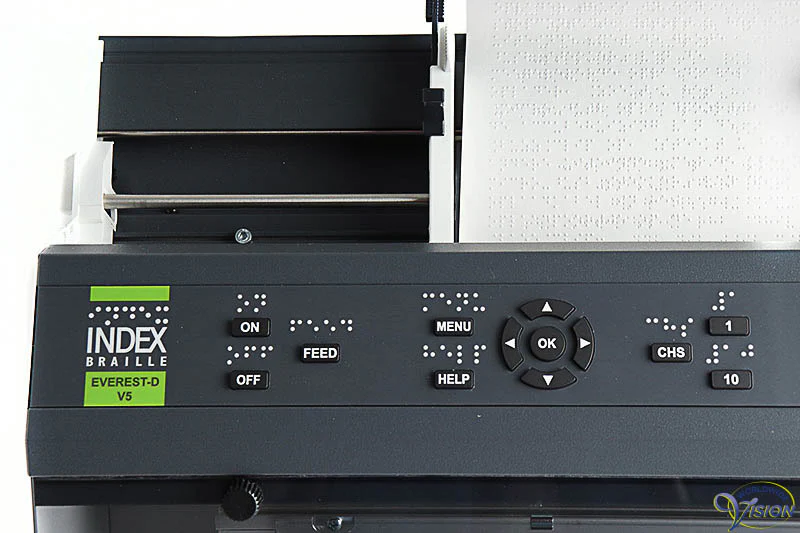
\includegraphics[width=0.4\linewidth]{printer.png}
\caption{INDEX BRAILLE Everest-D V5}
\label{fig:INDEX BRAILLE Everest-D V5}
\end{figure} \\

\subsubsection{Scanner configuration}
we used specific Scanner properties to remove any variations and ensure the persistence of high accuracy by supplying the preprocessing stage by the same properties of digitalized paper.\\

\noindent Source: Flatbed\\
Color format:	Grayscale\\
File type: JPG, PNG\\
Resolution (DPI): 100\\


    \clearpage
\subsection{Block Diagram }

\begin{figure}[!ht]
\centering
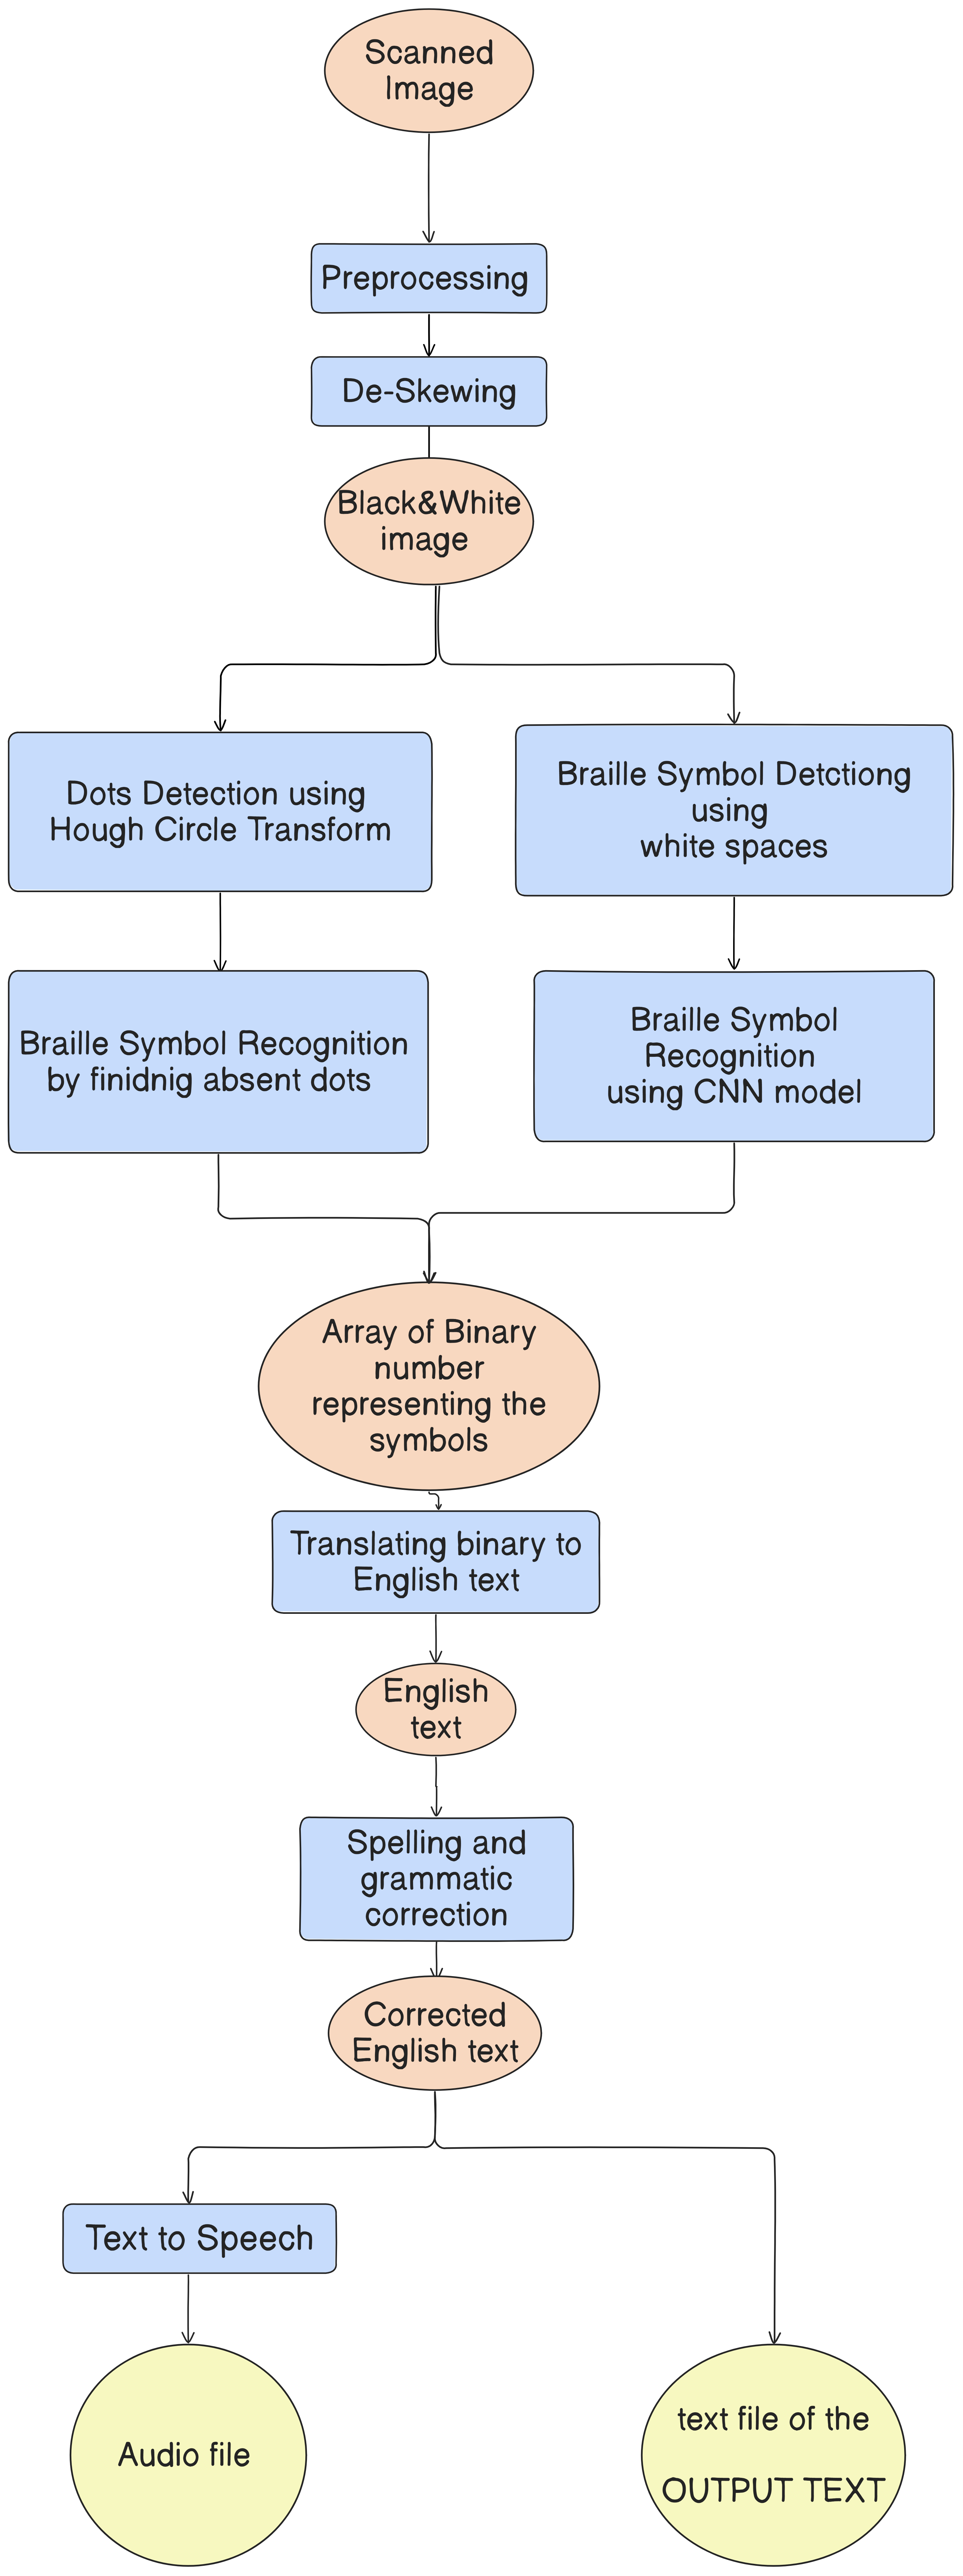
\includegraphics[width=0.55\linewidth]{BD.png}
\caption{Block Diagram}
\label{fig:Block Diagram}
\end{figure} \\

\newpage
The Block diagram, shown in Figure 3.2, illustrates the process of converting a scanned Braille image into readable and audible English text. Here's a step-by-step explanation:

\begin{enumerate}
    \item \textbf{Scanned Image}: The process begins with a scanned image of the Braille text using the scanner configuration mentioned above.

    \item \textbf{Preprocessing}: The scanned image undergoes several  filtering process which includes noise reduction and normalization. to prepare the image to be properly translated. this step reduces the complexity of  the next processes.

    \item \textbf{De-Skewing}: The image is de-skewed to correct any tilting that may have occurred during scanning, resulting in a properly aligned image.\\

\end{enumerate}
From this point, there are two paths for Braille symbol detection and recognition:\\

\paragraph{Path 1: Image Processing }
This path is illustrated as the right path of the block diagram shown in figure \ref{fig:Block Diagram}.

\begin{enumerate}
    \item \textbf{Dots Detection using Hough Circle Transform}: The Hough Circle Transform method is used to detect the centers of the circular shapes of Braille dots.

    \item \textbf{Braille Symbol Recognition by Finding Absent Dots}: A grid of all  possible symbols on a page is built. then the recognition process is done by comparing the grid to the detected Dots from the Hough circle transformation function. The presence or absence of dots in the recognized patterns decides  the Braille symbols.
\end{enumerate}

\paragraph{Path 2: CNN }
This path is illustrated as the left path of the block diagram shown in figure \ref{fig:Block Diagram}.

\begin{enumerate}
    \item \textbf{Braille Symbol Detection using White Spaces}: White spaces between the dots are used to detect the individual location of each Braille symbol.
    \item \textbf{Braille Symbol Recognition using CNN Model}: A Convolutional Neural Network (CNN) model is employed to recognize the Braille symbols from the detected patterns.\\
\end{enumerate}


After symbol recognition, both paths' output is a binary array of the braille symbols recognized as zeros and ones. The two paths then continue to the same post-recognition processes:

\begin{enumerate}

    \item \textbf{Translating Binary to English Text}: The binary numbers are translated into corresponding English text.
.
    \item \textbf{Spelling and Grammatical Correction}: The English text is corrected for any spelling and grammatical errors, resulting in corrected English text.
\end{enumerate}
Finally, the corrected English text can be output in two formats:

\begin{itemize}
    \item \textbf{Text to Speech}: The corrected English text is converted into an audio file.
    \item \textbf{Text File of the Output Text}: The corrected English text is saved as a text file.
\end{itemize}
This process allows for the conversion of Braille to both readable and audible formats, making the information accessible to a wider audience.

 
